%-%-%-%--%-%-%-%-%-%--%-%-%--%-%
% Author  : Tiago Chedraoui Silva
% License : GNU GPL v.3
% Title   : Mapa mental
% Tags    : mindmap, layers
%-%-%-%-%-%-%-%-%-%--%-%-%-%-%-%
\documentclass{article}
\usepackage{color}
\usepackage{tikz,times}
\usepackage[paperwidth=25cm,paperheight=16cm,left=1cm,top=1cm]{geometry}
\usetikzlibrary{mindmap,backgrounds}

\pagestyle{empty}
\begin{document}
\centering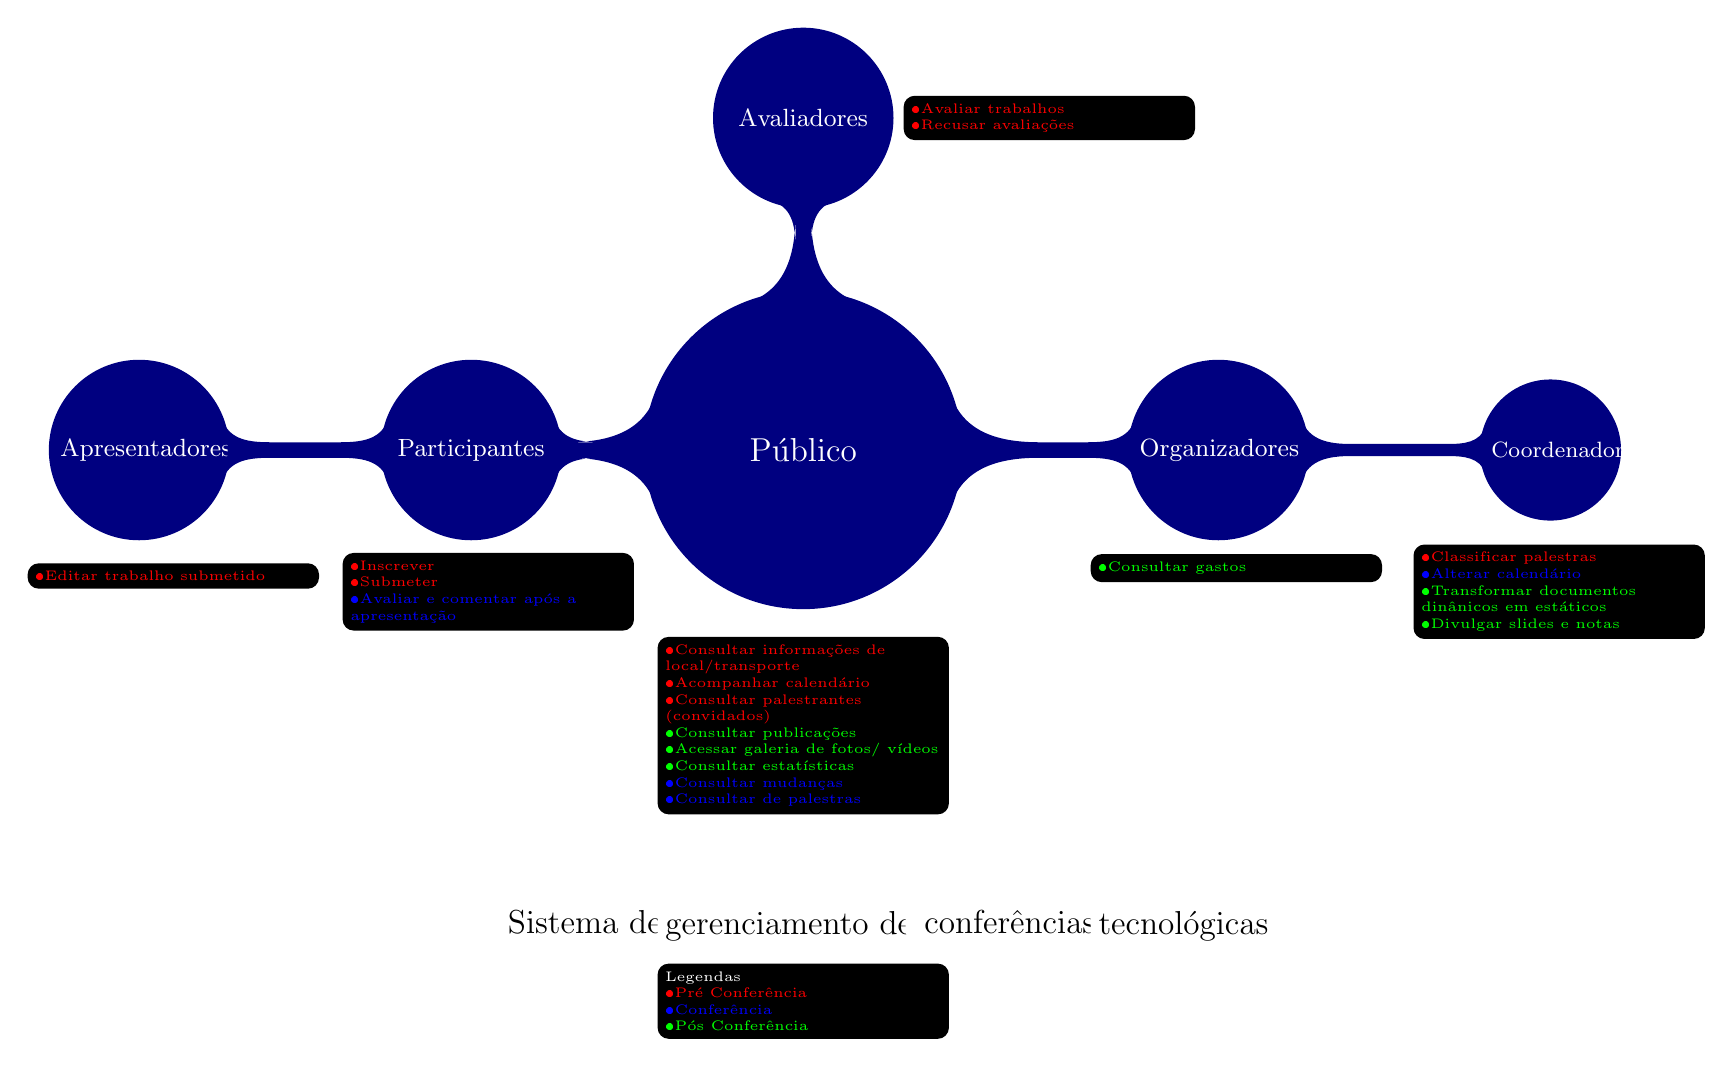
\begin{tikzpicture}[mindmap,
  level 1 concept/.append style={level distance=130,sibling angle=30},
  extra concept/.append style={color=blue!50,text=black},every annotation/.style={fill=black}]

  \begin{scope}[mindmap, concept color=blue!50!black, text=white,every annotation/.style={fill=black}]
    \node [concept](pub) at (0,-14.0)  {P\'ublico}
      child [grow=90, level distance=120] 
        {node [concept] (ava) {Avaliadores}}
    child [grow=0, level distance=150] 
        {node [concept] (org) {Organizadores}
	{ child [grow=0, level distance=120] 
	 {node [concept] (coo) {Coordenadores}}
	}   }
        child [grow=180, level distance=120] 
	{node [concept] (par) {Participantes}}
	{   child [grow=180, level distance=120] 
        {node [concept] (apr) {Apresentadores}} 
   
  };


%% Legenda


     \node [annotation,color=white,text=black] at (-2,-20)
      {\large{Sistema de}};

     \node [annotation,color=white,text=black] at (0,-20.05)
      {\large{gerenciamento de }};
  
 \node [annotation,color=white,text=black] at (3.15,-20)
      {\large{ confer\^encias}};
  \node [annotation,color=white,text=black] at (5.5,-20.05)
      {\large{tecnol\'ogicas}};



     \node [annotation] at (0,-21)
      {Legendas\\\textcolor{red}{\textbullet Pr\'e Confer\^encia} \\ \textcolor{blue}{\textbullet  Confer\^encia}\\\textcolor{green}{\textbullet P\'os Confer\^encia}};



%%avaliadores
     \node [annotation,right] at (ava.east)
      {\textcolor{red}{\textbullet Avaliar trabalhos \\ \textbullet Recusar avalia\c{c}\~oes}};


%%coordenadores
    \node [annotation] at (9.6,-15.8)
      {\textcolor{red}{\textbullet Classificar palestras} \\
\textcolor{blue}{\textbullet Alterar  calend\'ario}\\\textcolor{green}{\textbullet Transformar documentos din\^anicos em est\'aticos\\ \textbullet Divulgar slides e notas}};
 
%%Organizadores
   \node [annotation] at (5.5,-15.5)
      {\textcolor{green}{\textbullet Consultar gastos}};

%%apresentadores
    \node [annotation,left] at (-6,-15.6)
      {\textcolor{red}{\textbullet Editar trabalho submetido} };

    \node [annotation] at (0,-17.5)
      {\textcolor{red}{\textbullet Consultar informa\c{c}\~oes de local\slash transporte \\
 \textbullet Acompanhar calend\'ario\\
\textbullet Consultar palestrantes (convidados)}\\
\textcolor{green}{\textbullet Consultar publica\c{c}\~oes\\
\textbullet Acessar galeria de fotos/ v\'ideos\\\textbullet  Consultar estat\'isticas}
\\\textcolor{blue}{\textbullet Consultar  mudan\c{c}as\\
\textbullet Consultar de palestras } };


   \node [annotation] at (-4,-15.8)
      {\textcolor{red}{\textbullet Inscrever\\\textbullet Submeter}\\\textcolor{blue}{\textbullet Avaliar e comentar ap\'os a apresenta\c{c}\~ao }};

   
\end{scope}


% \begin{scope}[mindmap, concept color=white, text=white,every annotation/.style={fill=black}]
%    \node [concept](title) at (0,-20.0)  {P\'ublico};
% \end{scope} 
%   \node [annotation,text=white] at (title.north)
%{\huge{Sistema e gerenciamento de confer\^encias tecnol\'ogicas}};

  % Connections of researchers to applied subfields

  \begin{pgfonlayer}{background}
   % \draw [circle connection bar]
  % \draw [concept connection ]
   %  (ac) edge (prc-ling)
   %  (c-tr) edge (uimp)
   %  (c-err) edge (org);
  
 \end{pgfonlayer}
\end{tikzpicture}

\end{document}
